\let\negmedspace\undefined
\let\negthickspace\undefined
\documentclass[journal]{IEEEtran}
\usepackage[a5paper, margin=10mm, onecolumn]{geometry}
%\usepackage{lmodern} % Ensure lmodern is loaded for pdflatex
\usepackage{tfrupee} % Include tfrupee package

\setlength{\headheight}{1cm} % Set the height of the header box
\setlength{\headsep}{0mm}     % Set the distance between the header box and the top of the text

\usepackage{gvv-book}
\usepackage{gvv}
\usepackage{cite}
\usepackage{amsmath,amssymb,amsfonts,amsthm}
\usepackage{algorithmic}
\usepackage{graphicx}
\usepackage{textcomp}
\usepackage{xcolor}
\usepackage{txfonts}
\usepackage{listings}
\usepackage{enumitem}
\usepackage{mathtools}
\usepackage{gensymb}
\usepackage{comment}
\usepackage[breaklinks=true]{hyperref}
\usepackage{tkz-euclide} 
\usepackage{listings}
% \usepackage{gvv}                                        
\def\inputGnumericTable{}                                 
\usepackage[latin1]{inputenc}                                
\usepackage{color}                                            
\usepackage{array}                                            
\usepackage{longtable}                                       
\usepackage{calc}                                             
\usepackage{multirow}                                         
\usepackage{hhline}                                           
\usepackage{ifthen}                                           
\usepackage{lscape}
\begin{document}

\bibliographystyle{IEEEtran}
\vspace{3cm}

\title{1-1.4-9f}
\author{EE24BTECH11043 - Murra Rajesh Kumar Reddy}
% \maketitle
% \newpage
% \bigskip
{\let\newpage\relax\maketitle}

\renewcommand{\thefigure}{\theenumi}
\renewcommand{\thetable}{\theenumi}
\setlength{\intextsep}{10pt} % Space between text and floats


\numberwithin{equation}{enumi}
\numberwithin{figure}{enumi}
\renewcommand{\thetable}{\theenumi}

\textbf{Question}:\\
The point which divides the line segment joining the points $P(7,-6)$ and $Q(3,4)$ in the ratio $1:2$ internally lies in which quadrant?
\\
\textbf{Solution}:
\\
\textbf{Section Formula}: The line segment $A\brak{x_1,y_1}$ and $B\brak{x_2,y_2}$ is internally divided by the point $C\brak{x,y}$ in the ratio $m:n$ is given by
\\
\begin{align}
\centering
	C\brak{x,y} = \brak{\frac{mx_2+nx_1}{m+n},\frac{my_2+ny_1}{m+n}}
\end{align}
\\
\begin{figure}[h!]
	\centering
	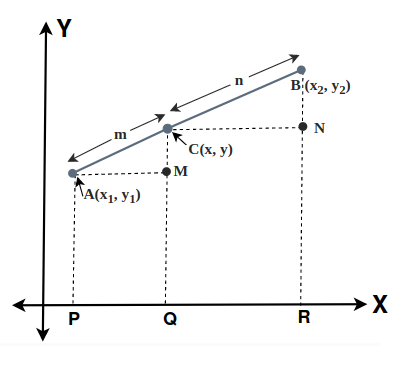
\includegraphics[width=0.7\linewidth]{figs/fig_2.png}
	\caption{Section Formula}
	\label{Section Formula}
\end{figure}
\\
Let $R\brak{x,y}$ be the point which divides the line segment $P\brak{7,-6}$ and $Q\brak{3,4}$ in the ratio $1:2$ internally 
\\
\newpage
From equation 0.1 $R\brak{x,y}$ is :
\\
\begin{align}
	R\brak{x,y} = \brak{\frac{1\times3+2\times7}{1+2},\frac{1\times4+2\times\brak{-6}}{1+2}}\\
	\implies R\brak{x,y} = \brak{\frac{17}{3},\frac{-8}{3}}
\end{align}

\end{document}


